\chapter{The Search for $\boldmath{t+p_\text{T}^\text{miss}}$}
\label{sec:mt}

In this chapter, we discuss the search for dark matter produced in association with a single top quark (``mono-top'').
Since the initial state of $pp$ collisions do not contain any appreciable contribution from top quarks, any process that produces a single top quark must involve some flavor violation.
In the Standard Model, any such process is heavily suppressed by off-diagonal elements of the CKM matrix.
The SM production mechanism for the mono-top signature (Fig.~\ref{fig:mt:tzq}) involves a $b$ quark in the final state, and thus does not couple the third generation with the first or second.
True production of mono-top must introduce some such coupling as an extension to the SM, in addition to one (or more) invisible particle to serve as a DM candidate.

\begin{figure}[!ht]
    \begin{center}
        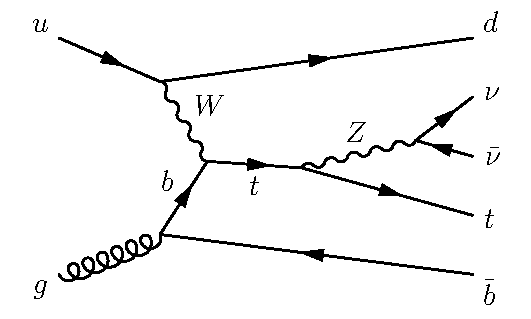
\includegraphics[width=0.5\textwidth]{figures/monotop/diagrams/tzq.pdf}
        \caption{Production of mono-top in the SM, in which a top quark is produced in addition to a $Z$ boson and bottom quark. The $Z$ decays to neutrinos, providing large \ptmiss.}
        \label{fig:mt:tzq}
    \end{center}
\end{figure}

To illustrate how beyond-SM physics can produce this final state, we introduce two DM models: a flavor-changing neutral current $V$ and a charged, colored scalar $\phi$.
These models will also be used to benchmark the sensitivity of the analysis.
However, it should be emphasized that the search is motivitated and designed agnostically, without reliance on any specific model; the assumption is that the mono-top final state alone is indicative of new physics, regardless of the specific production mechanism.

The FCNC $V$ is assumed to couple to a fermionic DM candidate $\chi$. 
A partial Lagrangian of the interaction terms is given by:
\begin{equation}
\mathcal{L}_\text{int}=  V_\mu  \overline\chi \gamma^\mu (  g^V_{\chi} + g^A_{\chi} \gamma_5 ) \chi
                           + \overline{q}_u \gamma^\mu
                           ( g^V_u + g^A_u \gamma_5 ) q_u V_\mu
                           + \overline{q}_{d} \gamma^\mu
                           (  g^V_{d} + g^A_{d} \gamma_5 ) q_d V_\mu
                           + \text{h.c.},
    \label{eq:Lfcnc}
\end{equation}
The model comes with 22 free parameters, broadly organized in three sets:
\begin{itemize}
    \item The masses $m_V$ and $m_\chi$. (2)
    \item The couplings $g_\chi^V$ and $g_\chi^A$. These, respectively, control the strength of the vector and axial interactions between $V$ and $\chi$. (2)
    \item The four coupling matrices $g_{q}^{X}$, where $q=u,d$ and $X=V,A$. 
          As before, $X$ determines the type of spin-1 interaction. 
          In principle, different coupling strengths can be permitted for up- and down-type quarks, so this indexed by $q$. 
          Each $g_{q}^{X}$ is a $3\times3$ matrix, cross-coupling the three quark generations. 
          To preserve $\mathrm{SU}(2)_\mathrm{L}$ symmetry, we require $g_u^V - g_u^A = g_d^V - g_d^A$. ($3\times6=18$)
\end{itemize}

It is the $g_{u,d}^{V,A}$ that determine whether the model can produce mono-top, or mono-bottom, or mono-up, etc. 
If $g_{u,d}$ is strongly diagonal (i.e. strongest couplings are within generations), then mono-light quark production will dominate, resulting in the mono-jet final state (Fig~\ref{fig:mt:fcncdiaga}).
On the other hand, if we assume the only non-zero elements are those that couple the first and third generations, then mono-top production at the LHC is the best way to probe this model (Fig~\ref{fig:mt:fcncdiagb}).
It is this latter choice that will be made in the rest of this chapter; other choices are best probed using a combination of multiple DM channels, which is left as future work.
Furthermore, to respect $\mathrm{SU}(2)_\mathrm{L}$ symmetry, we make the assumption that $g_u^V = g_d^V$ and $g_u^A = g_d^A$.

\begin{figure}[!ht]
    \begin{center}
        \begin{subfigure}[t]{0.49\textwidth}
            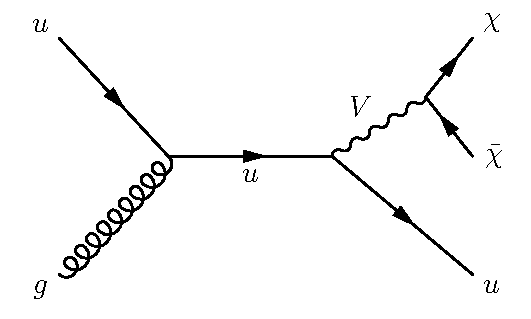
\includegraphics[width=\textwidth]{figures/monotop/diagrams/mj.pdf}
            \caption{If the coupling matrix is dominated by diagonal elements, mono-jet production is enhanced.}
            \label{fig:mt:fcncdiaga}
        \end{subfigure}
        \begin{subfigure}[t]{0.49\textwidth}
            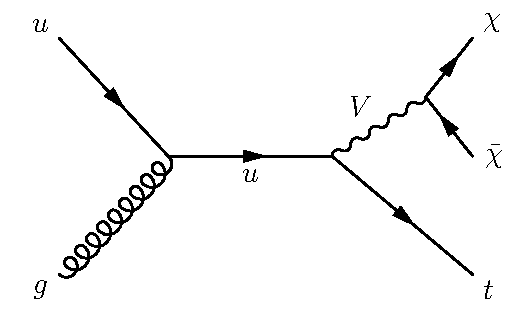
\includegraphics[width=\textwidth]{figures/monotop/diagrams/fcncb.pdf}
            \caption{If $(g_{u}^{V,A})_{ij} \approx \delta_{i1}\delta_{j3} + \delta_{i3}\delta_{j1}$, then mono-top production is dominant.}
            \label{fig:mt:fcncdiagb}
        \end{subfigure}
        \caption{Possible DM production at the LHC, assuming a simplified spin-1 extension to the SM.}
        \label{fig:mt:fcncdiag}
    \end{center}
\end{figure}

In the second benchmark model, the charged, colored scalar $\phi$ couples to down-type quarks, or to a fermionic DM candidate $\psi$ and a top quark.
The interaction terms of the Lagrangian is given by:
\begin{equation}
    \mathcal{L}_\text{int} = \phi\overline{{d}}_i^C[(a_{q})^{ij}+(b_{q})^{ij}\gamma^5]{d}_j+\phi\overline{{t}}[a_{\psi}+b_{\psi}\gamma^5]\psi+\text{h.c.}
\end{equation}
There are 16 free parameters in this model, broadly organized in three categories:
\begin{itemize}
    \item The masses $m_\phi$ and $m_\psi$. (2)
    \item The couplings at the $\phi \bar{t} \psi$ vertex $a_\psi$ and $b_\psi$, which respectively control the strength of the scalar and pseudoscalar interactions. (2)
    \item The couplings at the $\phi \bar{d_i} d_j$ vertex $a_q^{ij}$ and $b_q^{ij}$ where $i,j=1,2,3$. Again, $a$ and $b$ refer the scalar and pseudoscalar couplings, respectively. (12)
\end{itemize}
In this model, mono-top production primarily occurs through the resonant decay of $\phi$ to $\psi$ and $t$, as shown in Fig~\ref{fig:mt:resdiag}.

\begin{figure}[!ht]
    \begin{center}
        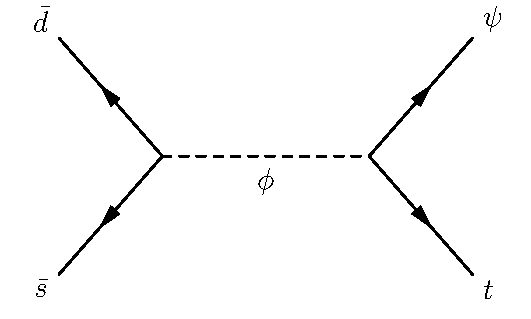
\includegraphics[width=0.5\textwidth]{figures/monotop/diagrams/resonant.pdf}
        \caption{Possible DM production at the LHC, assuming the existence of a charged, color scalar that couples to DM and the top quark.}
        \label{fig:mt:resdiag}
    \end{center}
\end{figure}

The two benchmark models show markedly different spectra in Fig~\ref{fig:mt:shapes}, motivating their use to test different modes of mono-top production.
The FCNC produces a falling \ptmiss~distribution, whereas the scalar resonance produces a \ptmiss~distribution peaking at approximately $m_\phi / 2$. 

\begin{figure}[!ht]
    \begin{center}
        \begin{subfigure}[t]{0.49\textwidth}
            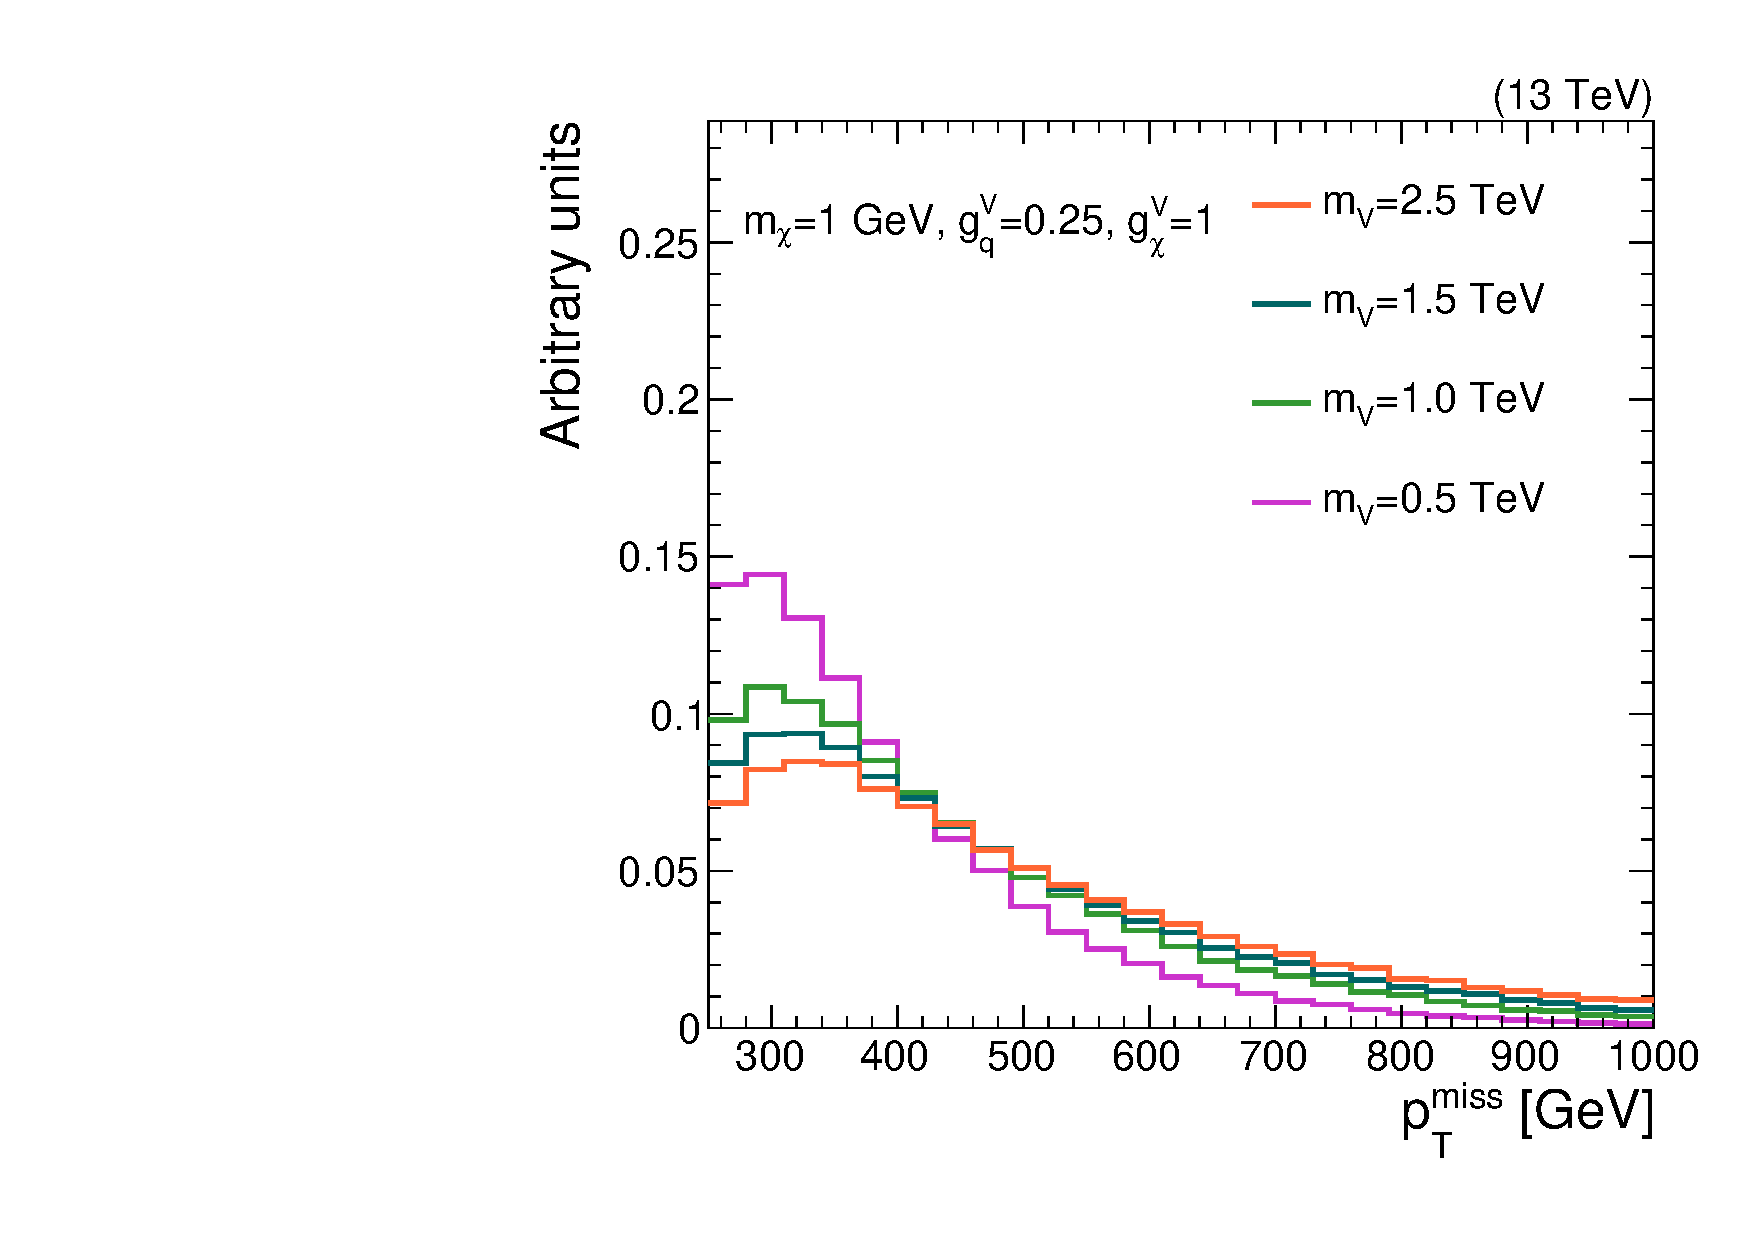
\includegraphics[width=\textwidth]{figures/monotop/diagrams/fcnc_pfmet.pdf}
            \caption{FCNC}
        \end{subfigure}
        \begin{subfigure}[t]{0.49\textwidth}
            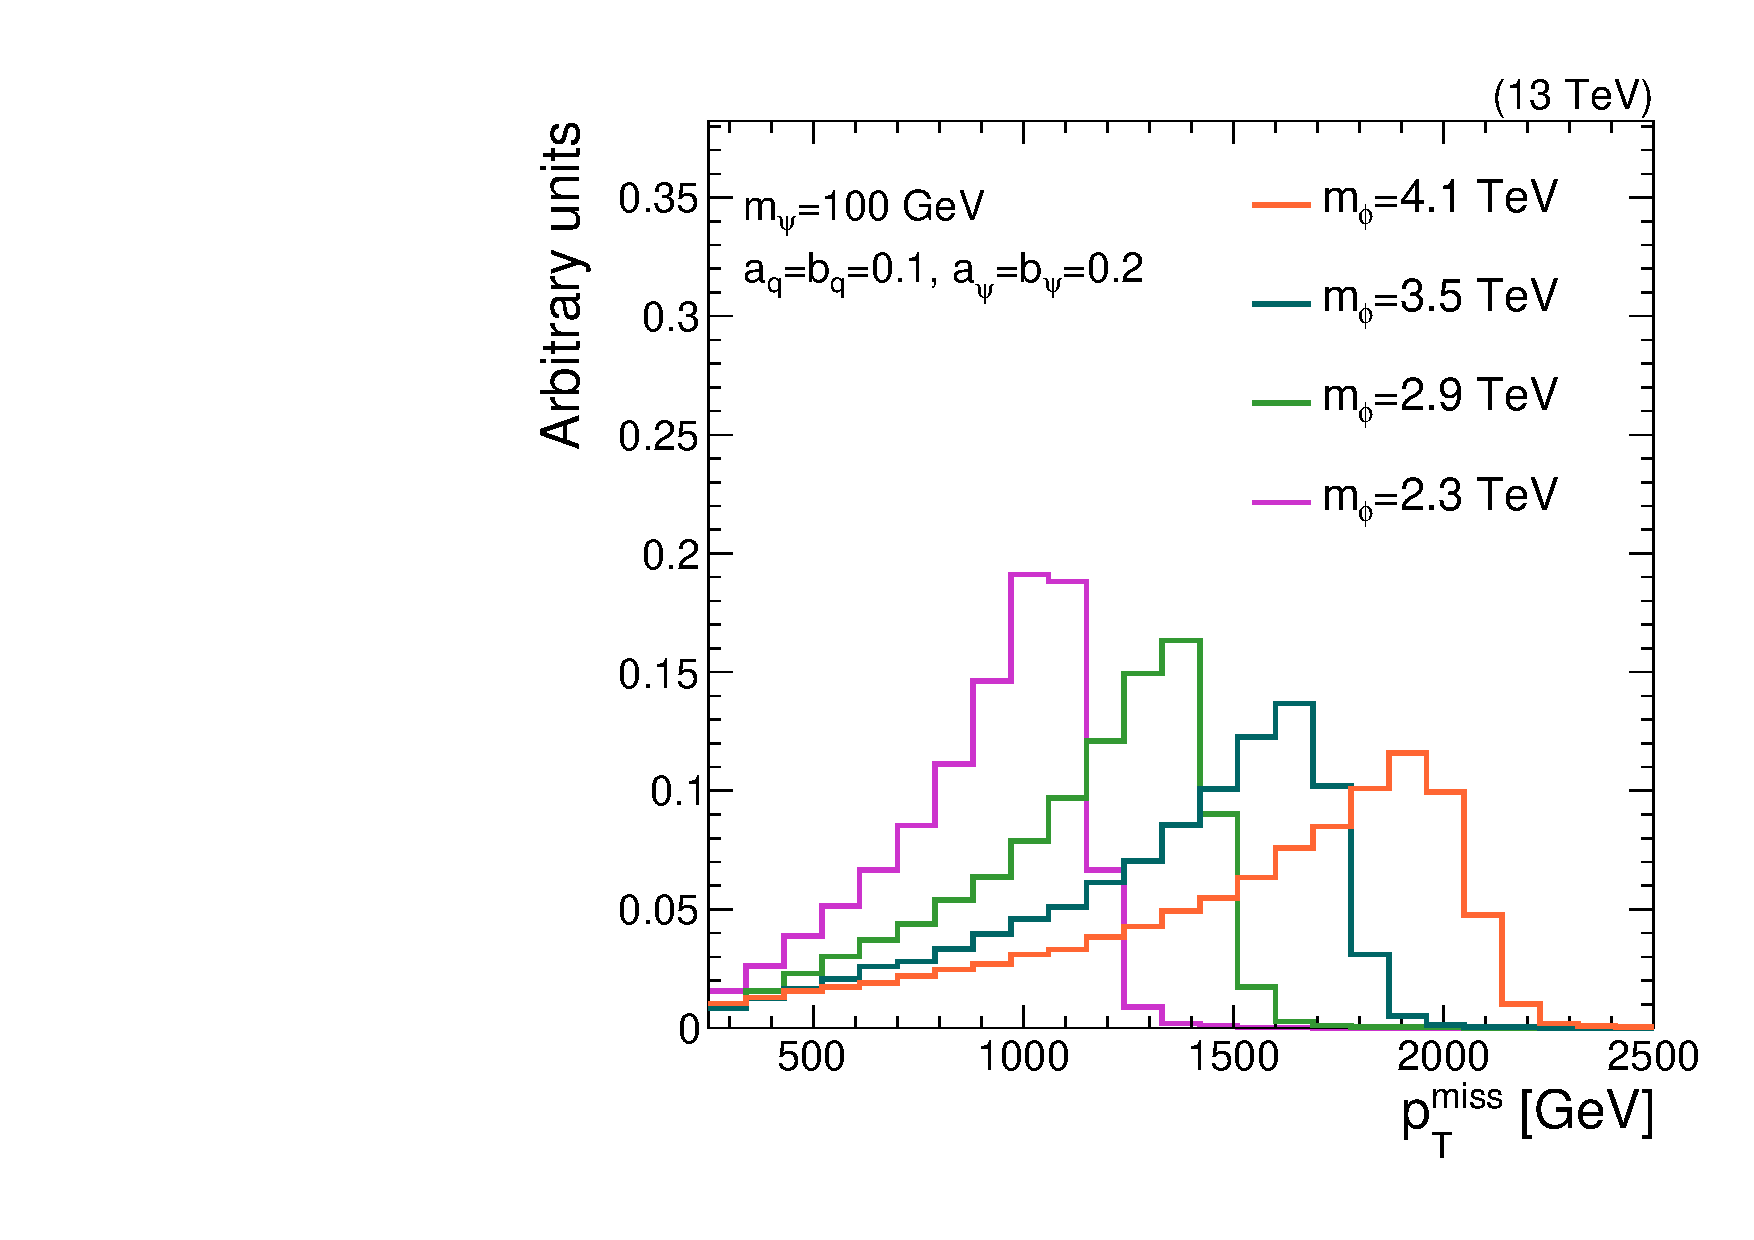
\includegraphics[width=\textwidth]{figures/monotop/diagrams/res_pfmet.pdf}
            \caption{Scalar resonance}
        \end{subfigure}
        \caption{Spectra of DM (missing) momentum under various signal hypothesis.}
        \label{fig:mt:shapes}
    \end{center}
\end{figure}

\clearpage

\section{Signal selection}
\label{sec:mt:sel}

When looking at events that pass a simple set of criteria (moderate $\ptmiss$ and one CA15 jet), it is clear (Fig~\ref{fig:mt:bkgshapes}) that the highest signal sensitivity is found in regions of high $\ptmiss$ and jet $\pt$.
The three primary background processes are:
\begin{itemize}
    \item $Z\rightarrow\nu\nu$. When the $Z$ is produced in association with one or more jets, the jet system can (with low probability) pass the criteria used to select a top jet. The neutrinos manifest as $\ptmiss$.
    \item $W\rightarrow\ell\nu$. As in the case of the $Z$, additional jets can mimic the signature of a top jet. Typically, the charged lepton in the final state is vetoed, but if it is out of acceptance ($e,\mu$) or fails ID criteria ($\tau_\mathrm{h}$), then it is not identified. 
    \item $t\bar{t} \rightarrow bq\bar{q}' + \bar{b}\ell\nu$. As in the case of the $W$, a charged lepton in the final state may not be properly identified. Unlike the previous two processes, a semi-leptonic $t\bar{t}$ event contains a real hadronic top quark decay. 
\end{itemize}

\begin{figure}[!ht]
    \begin{center}
        \begin{subfigure}[t]{0.49\textwidth}
            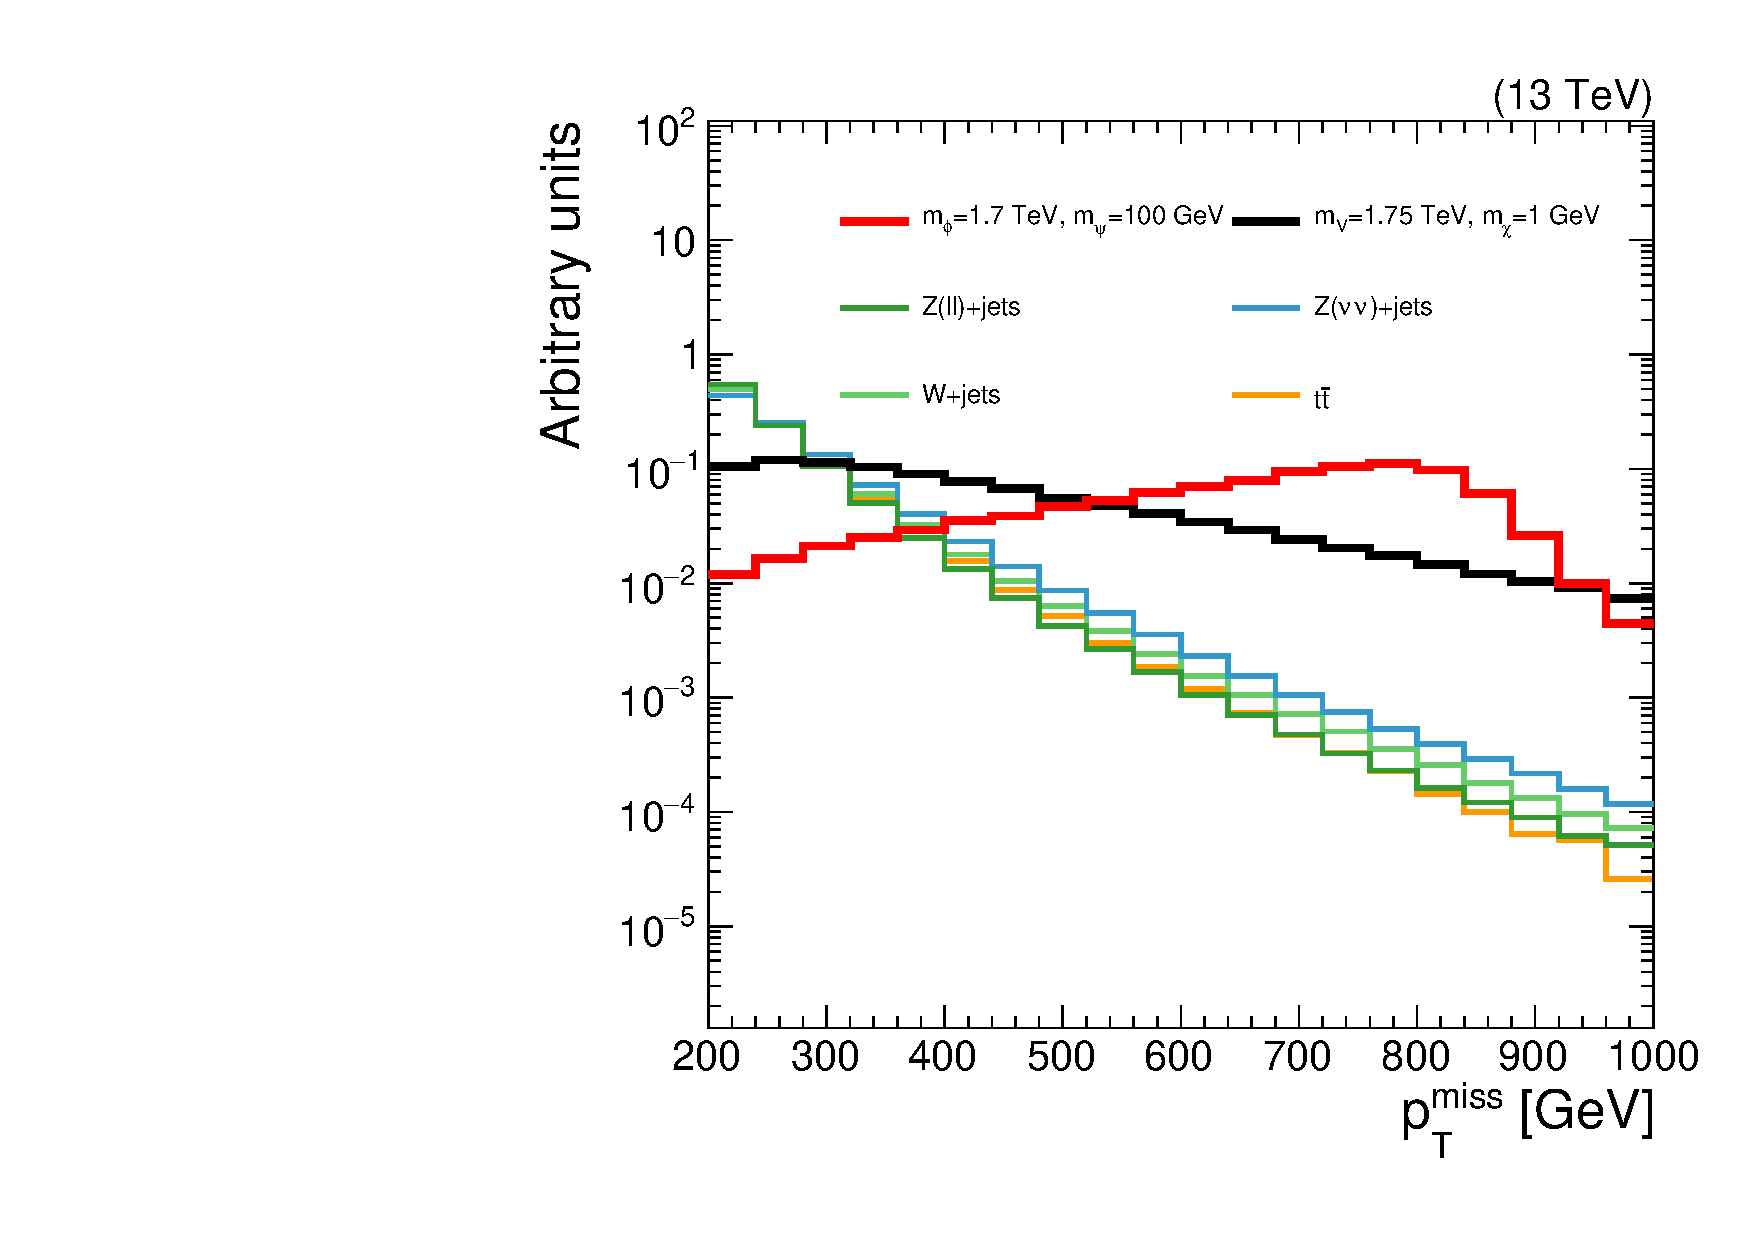
\includegraphics[width=\textwidth]{figures/monotop/shapes/signal_pfmet_logy.pdf}
            \caption{Missing momentum}
        \end{subfigure}
        \begin{subfigure}[t]{0.49\textwidth}
            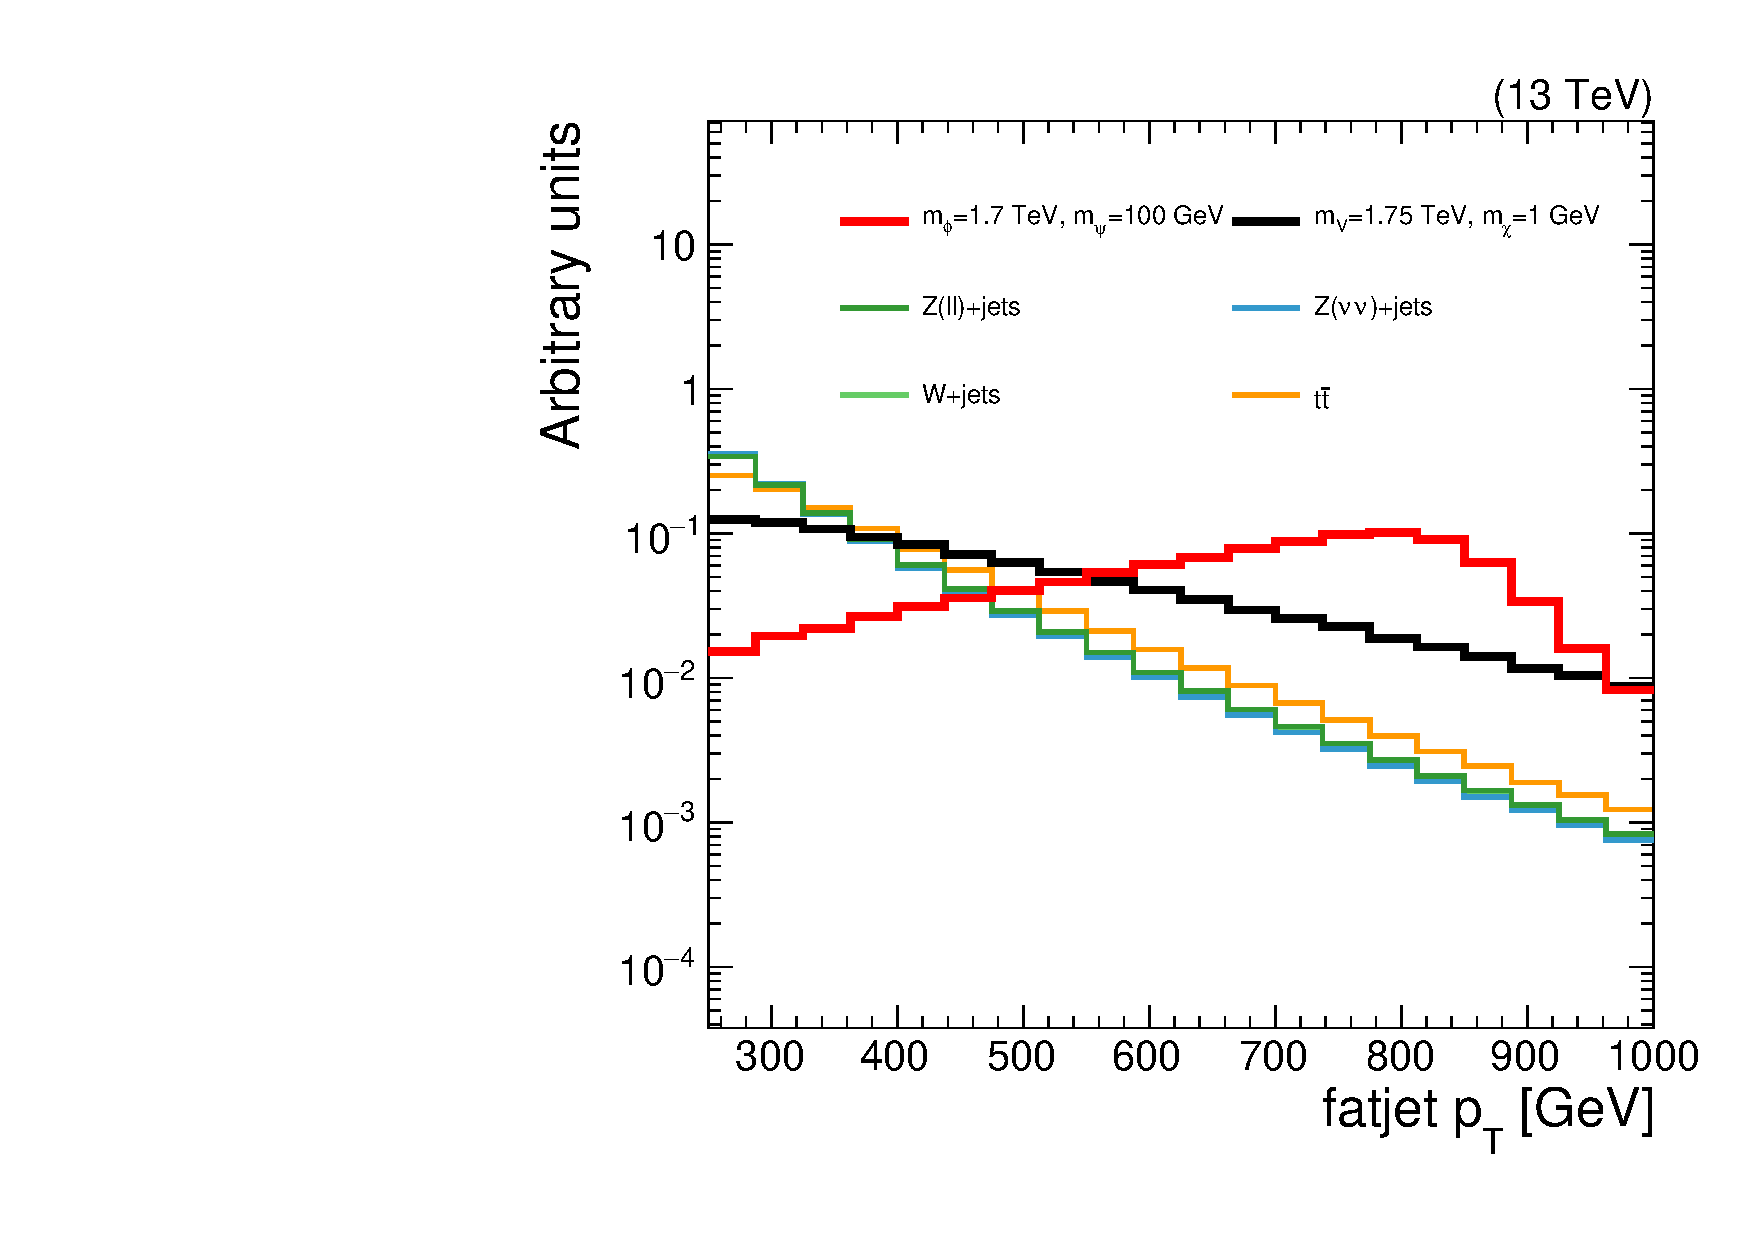
\includegraphics[width=\textwidth]{figures/monotop/shapes/signal_fjPt_0__logy.pdf}
            \caption{Jet $\pt$}
        \end{subfigure}
        \caption{Comparison of missing and jet momenta in various backgrounds and signal models.}
        \label{fig:mt:bkgshapes}
    \end{center}
\end{figure}

Events in the signal regions (SRs) are then selected according to Table~\ref{tab:mt:cuts}, chosen to be consistent with the signal topology while mitigating the aforementioned SM backgrounds.
As described in Section~\ref{sec:jets:combined}, two working points (WPs) are defined for the top ID BDT.
The signal events (passing all other selection criteria) are partitioned into a ``loose'' SR and a ``tight'' SR on the basis of which WP the top candidate jet satisfies. 

\begin{table}[!ht]
    \caption{Criteria used to select events for the mono-top search signal regions. Note that two SRs are defined, based on the BDT score.}
    \label{tab:mt:cuts}
    \begin{tabular}{p{0.4\textwidth}p{0.6\textwidth}}
        Criterion & Notes \\ 
        \hline 
        \hline 
        $\ptmiss>250$ GeV & Signal events should have large missing momentum. Exact threshold is chosen to maximize online trigger efficiency. \\ 
        1 CA15 jet with $\pt>250$ GeV & Top quark candidate. Recoils against $\ptmiss$, so threshold is set at $250$ GeV. \\ 
        CA15 jet $110 < m_\mathrm{SD} < 210$ GeV & Consistency with top quark mass. \\ 
        At least one $b$-tagged sub-jet & Identifying $B$ hadron produced from top decay/hadronization. \\ 
        \hline 
        No identified $e,\mu,\tau_\mathrm{h}$ & Suppress $W$+jet and $t\bar{t}$ processes. \\ 
        No identified $\gamma$ & Suppress $\gamma$+jet processes. \\ 
        \hline 
        $\min_\mathrm{jets}\Delta\phi(\mathrm{jet},\ptmiss) > 0.5$ & Remove events with large $\ptmiss$ caused by mismeasured jets. \\ 
        \hline 
        CA15 jet BDT & Identifying top decay structure. If the jet passes the tight WP, it is placed in the ``tight'' SR. Otherwise, if it only passes the loose WP, it is placed in the ``loose'' SR.\\ 
    \end{tabular}
\end{table}

Figure~\ref{fig:mt:prefit_signals} shows the $\ptmiss$ distributions, as predicted by MC and as observed in collected data, in the two signal regions.

\begin{figure}[!ht]
    \begin{center}
        \begin{subfigure}[t]{0.49\textwidth}
            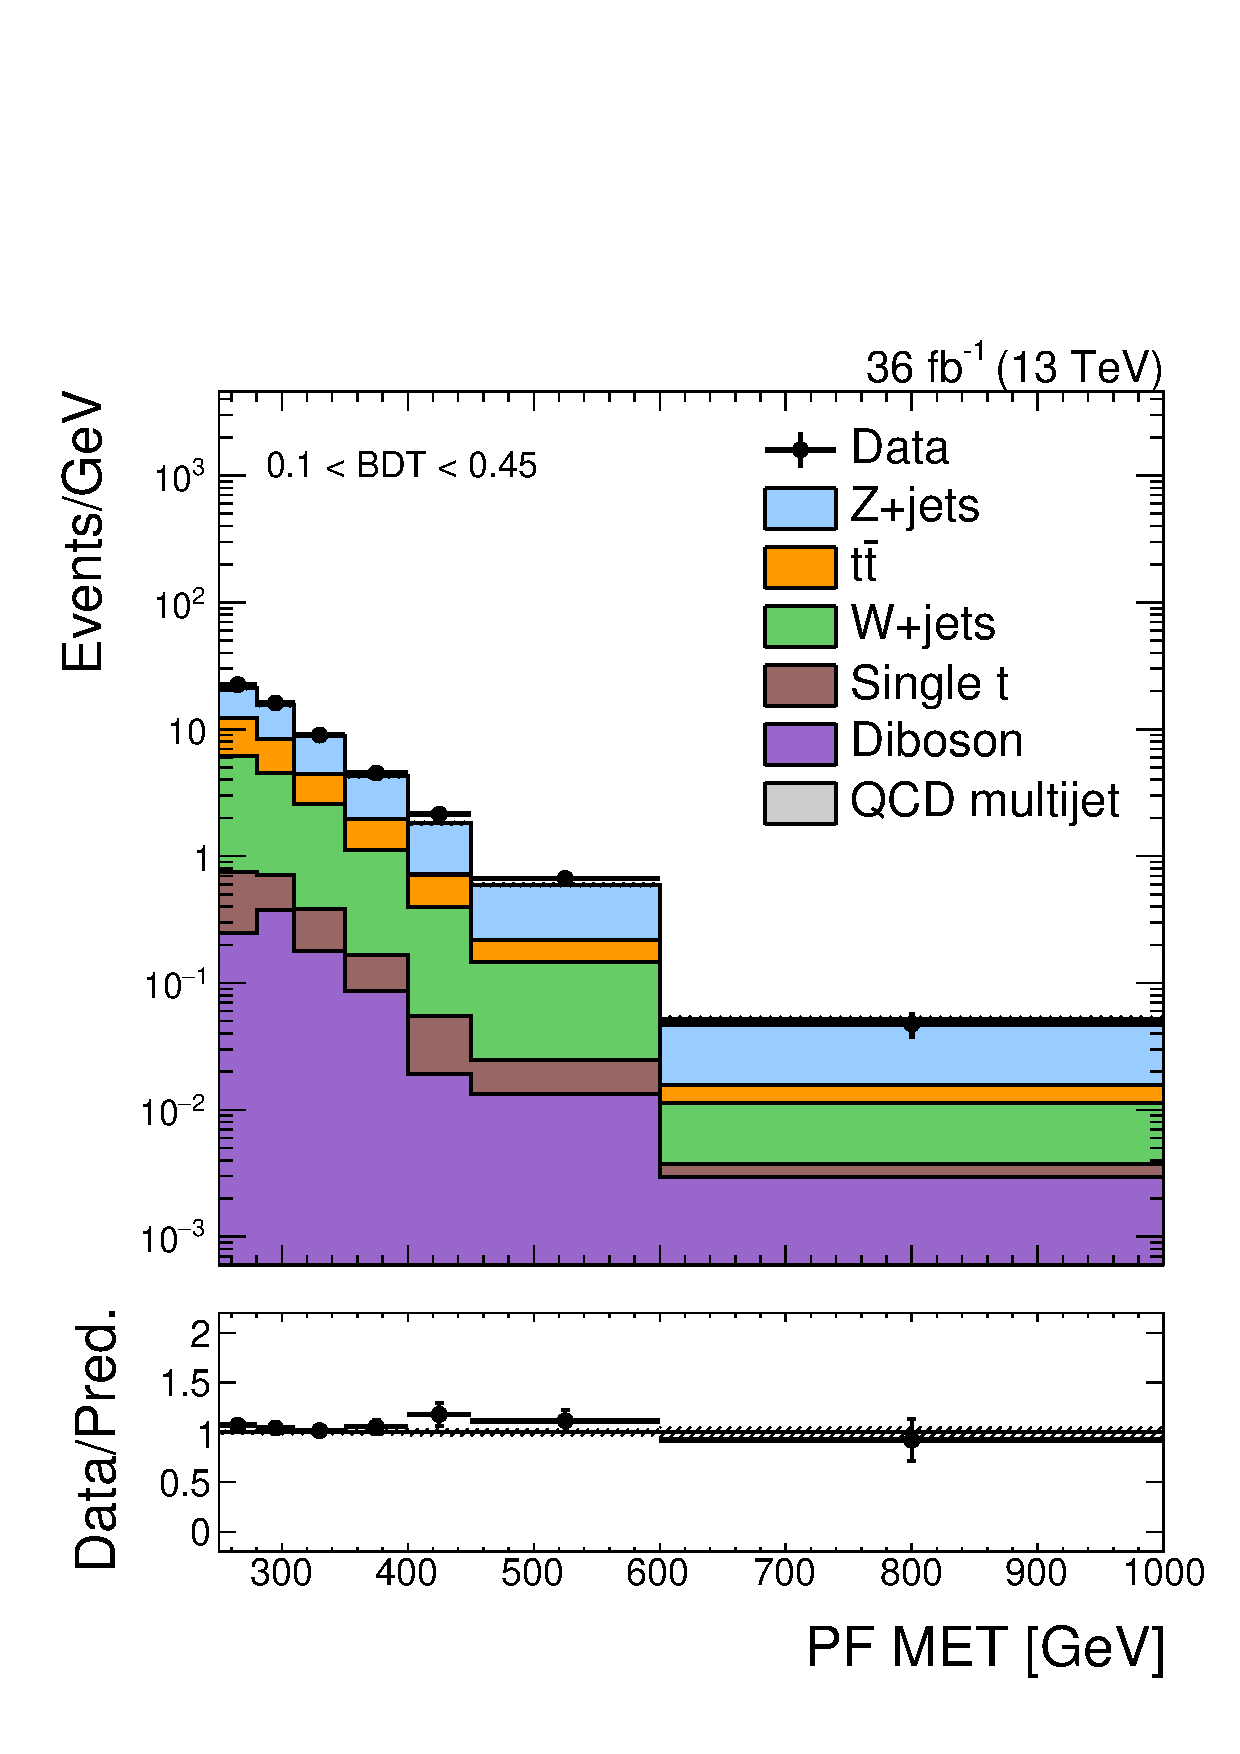
\includegraphics[width=\textwidth]{figures/monotop/prefit/signal_loose_pfmet_logy.pdf}
            \caption{Loose SR}
        \end{subfigure}
        \begin{subfigure}[t]{0.49\textwidth}
            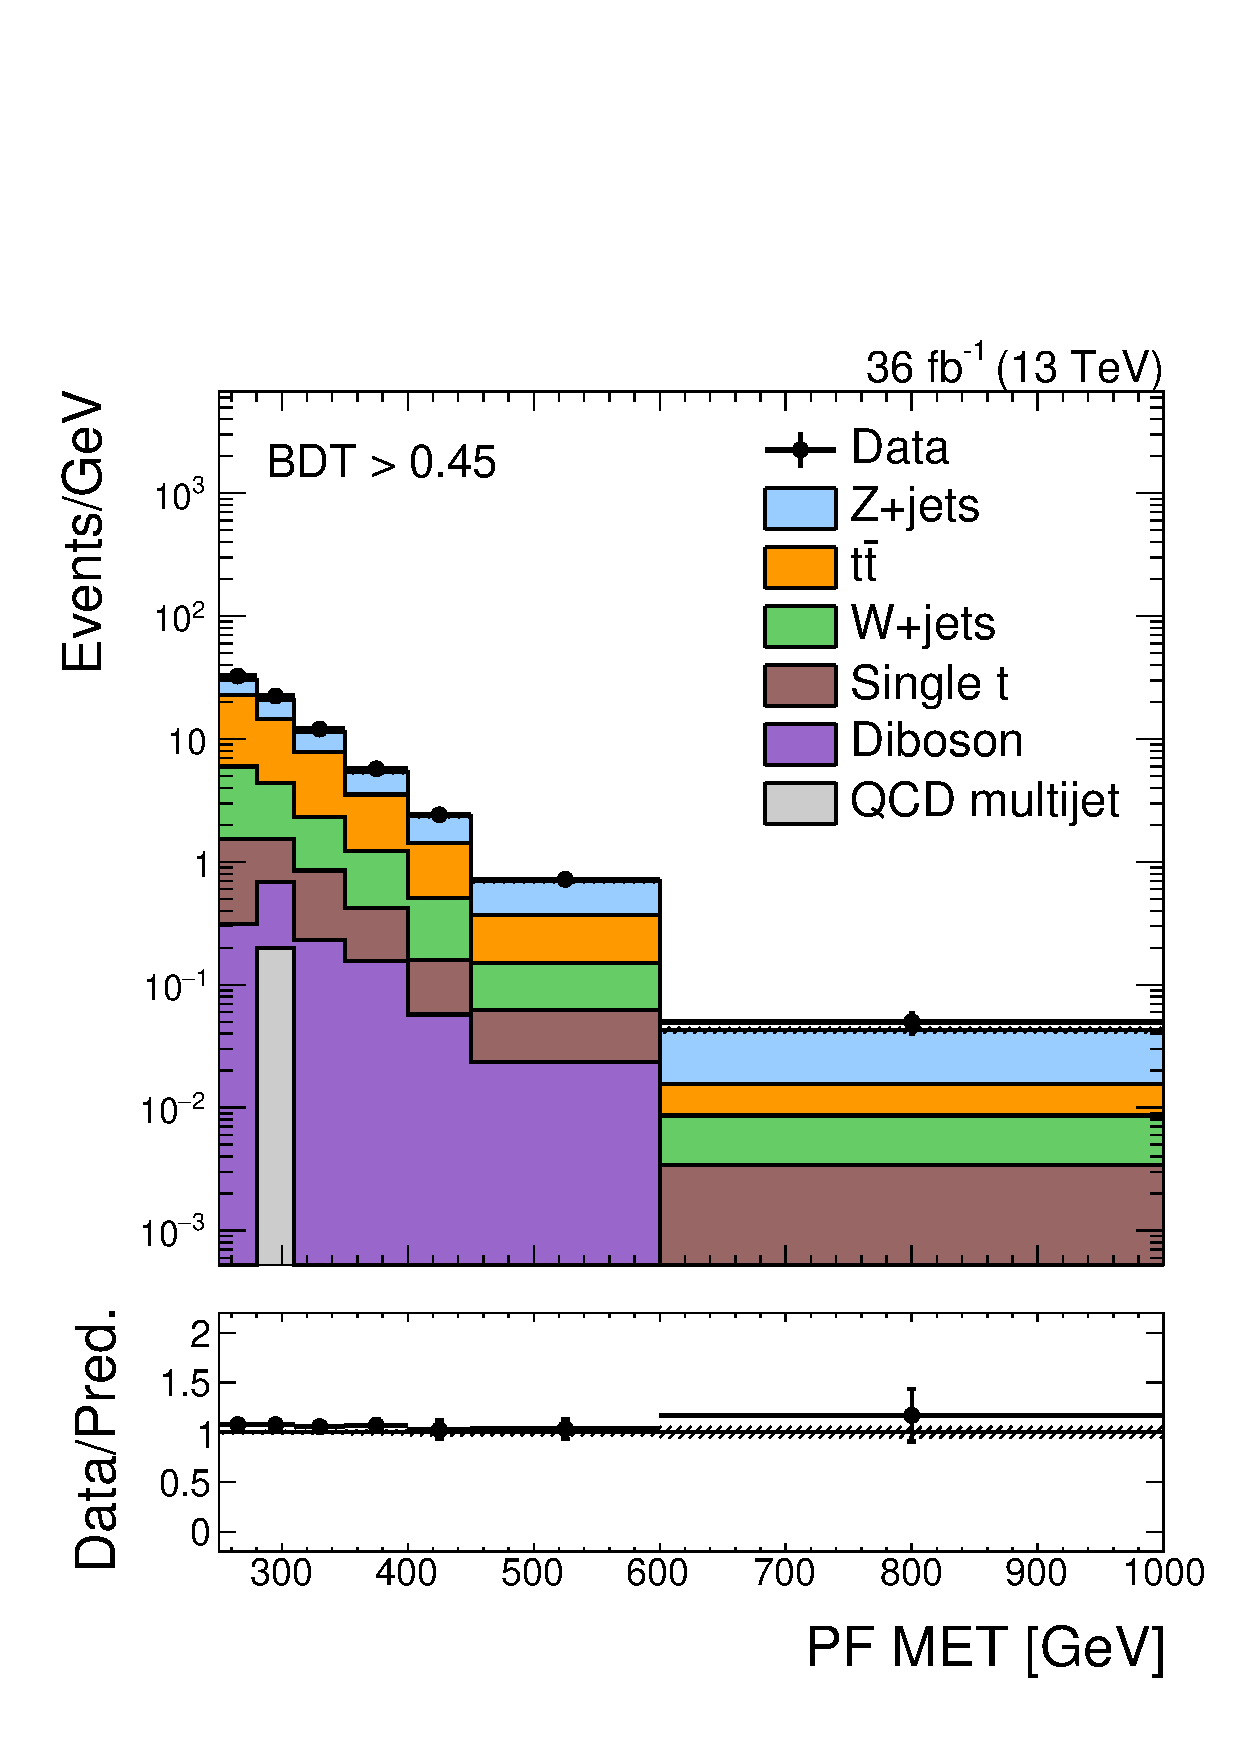
\includegraphics[width=\textwidth]{figures/monotop/prefit/signal_tight_pfmet_logy.pdf}
            \caption{Tight SR}
        \end{subfigure}
        \caption{$\ptmiss$ distributions in the two mono-top signal regions.
                 The bottom section of each figure shows the ratio of the data and the prediction.
                 The only uncertainties plotted in these figures are those arising from Poisson fluctations in data (black bars) and MC (grey band).}
        \label{fig:mt:prefit_signals}
    \end{center}
\end{figure}

\clearpage

\section{Background estimation}
\label{sec:mt:bkg}

Searching for DM amounts to looking for an excess of data events over the SM prediction at large values of $\ptmiss$.
Therefore, the $\ptmiss$ distribution of the three primary SM backgrounds described in Section~\ref{sec:mt:sel} must be predicted with small uncertainty.
The MC simulation provides a reasonable description of the data, but the theoretical uncertainties inherent in the MC (primarily due to higher-order QCD effects) can range up to $15\%$.
To reduce the prediction uncertainty further, a ``data-driven'' approach is used to estimate the SM processes in the SR.
In this context, ``data-driven'' refers to the use of control data (i.e. data that cannot contain signal) to directly estimate or supplement the estimation of SM processes in the SR.

\subsection{Visible final states to constrain invisible final states}

As a starting point, let us tackle the estimation of $Z\rightarrow\nu\nu$ in the SR.
Since the momentum imbalance (up to experimental effects) in a $Z\rightarrow\nu\nu$ event is just the transverse momentum of the $Z$ boson ($\pt^Z$), we must estimate $\pt^Z$.
To good approximation, the $\pt^Z$ distribution is independent of the decay mode of the $Z$ boson.
Therefore, it is natural to estimate $\ptmiss(Z\rightarrow\nu\nu)$ by measuring $\pt^Z(Z\rightarrow\mu\mu)$, as muons are easily identifiable and reconstructible. 

However, there is one important distinction between $\nu\nu$ and $\mu\mu$ events.
In the latter, $\pt^Z$ can be directly measured, whereas in the former it must be inferred through a momentum imbalance.
Effects like jet energy scale and acceptance can impact $\ptmiss$, but not $\pt^{\mu\mu}$. 
Therefore, instead of directly measuring $\pt^{\mu\mu}$ in $\mu\mu$ events, we define and use the hadronic recoil $U$:
\begin{equation}
    \vec{U} = \vec{\ptmiss} + \sum_{\mu} \vec{\pt}_\mu + \sum_{e} \vec{\pt}_e + \sum_\gamma \vec{\pt}_\gamma
\end{equation}
In the SR (where there are no $e,\mu,\gamma$), $U = \ptmiss$.
In $Z\rightarrow\mu\mu$ events, $U$ mimics the momentum imbalance, if we had pretended the identified muons did not exist when computing $\ptmiss$. 
Therefore, $U$ is an exact analogy for $\ptmiss$ in the SR.
Figure~\ref{fig:mt:zvsz} makes the same argument in a schematic fashion. 

\begin{figure}[!ht]
    \begin{center}
        \begin{subfigure}[t]{0.49\textwidth}
            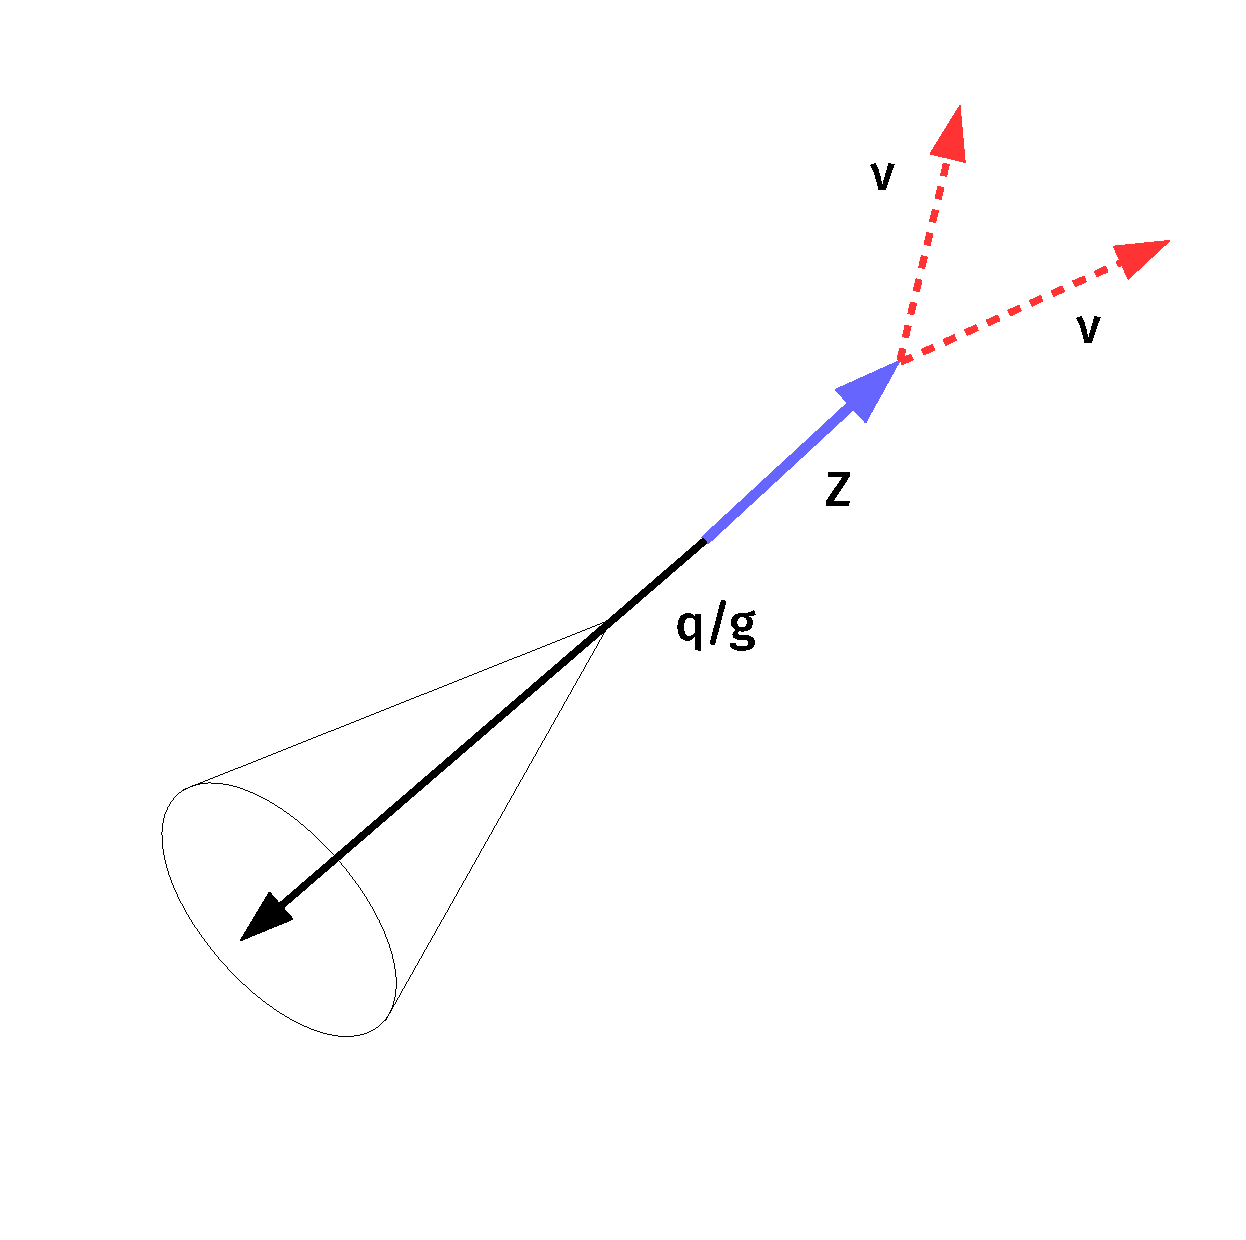
\includegraphics[width=\textwidth]{figures/monotop/diagrams/zsr.pdf}
            \caption{$Z\rightarrow\nu\nu$}
        \end{subfigure}
        \begin{subfigure}[t]{0.49\textwidth}
            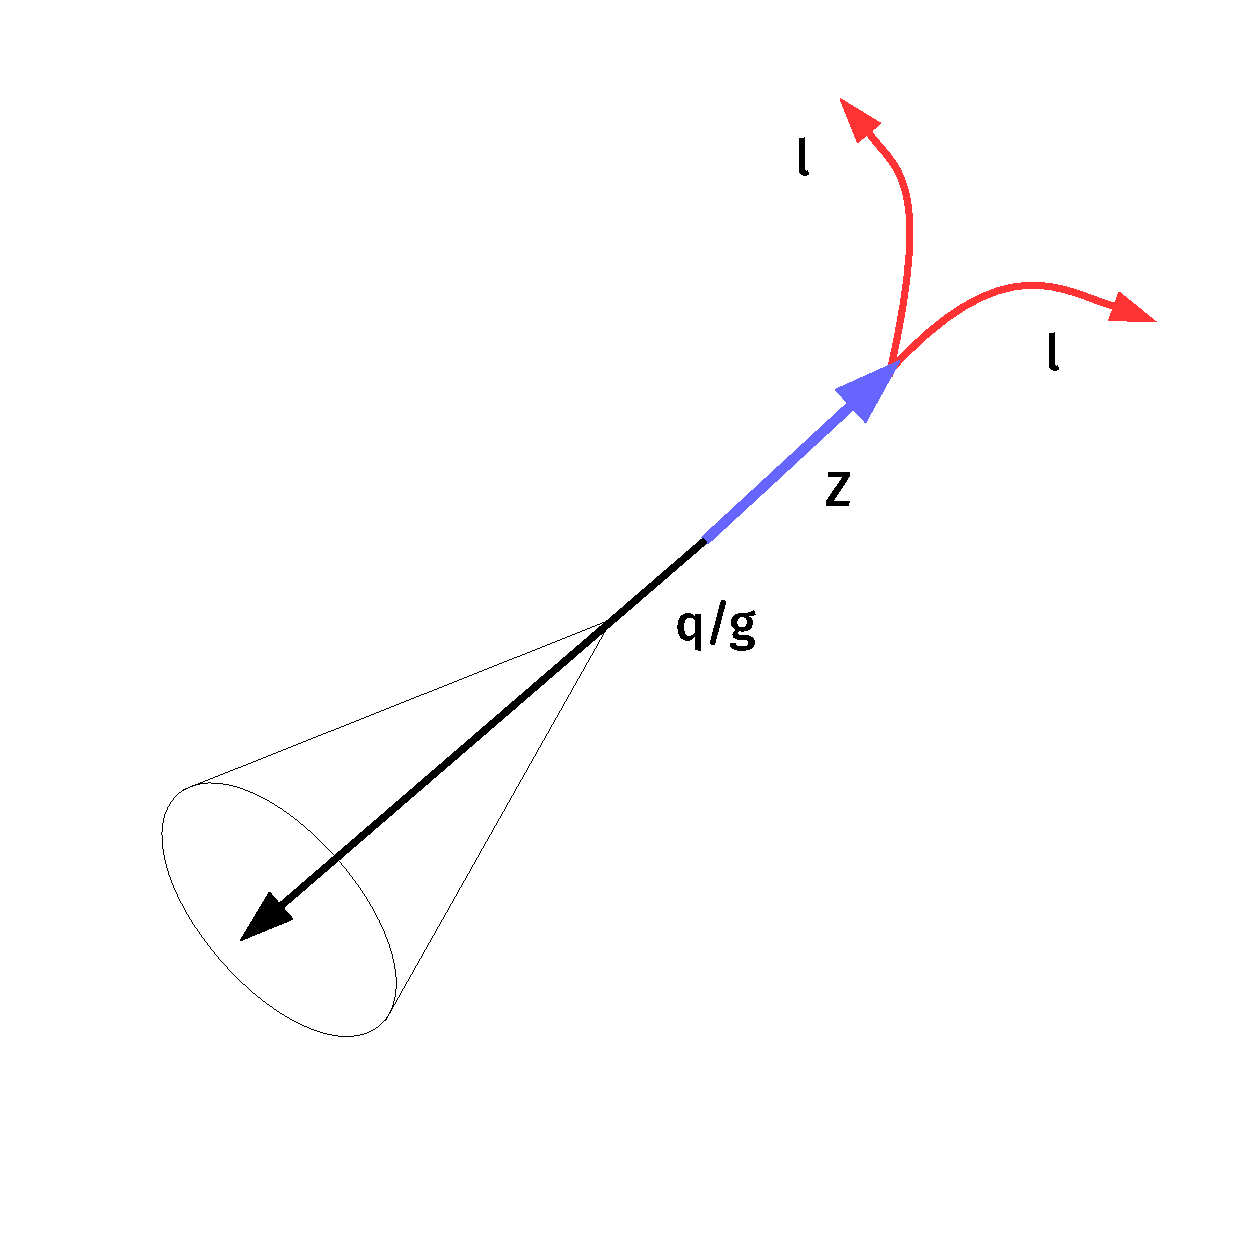
\includegraphics[width=\textwidth]{figures/monotop/diagrams/zcr.pdf}
            \caption{$Z\rightarrow\mu\mu$}
        \end{subfigure}
        \caption{Schematic representation of two $Z$ decay modes: to neutrinos (as in the SR) and to muons (as in the CRs).
                 Note that in both cases, $U$ is sensitive to the same effects arising from the measurement of the jet recoiling against the $Z$ boson, whereas $\pt^{\mu\mu}$ is largely invariant of the jet.}
        \label{fig:mt:zvsz}
    \end{center}
\end{figure}

Table~\ref{tab:mt:zmm_cuts} describes the criteria used to define events in the ``$\mu\mu$'' control regions (CRs). 
Figure~\ref{fig:mt:prefit_dimuons} shows the distribution of $U$ in these CRs. 

\begin{table}[!ht]
    \caption{Criteria used to select events for the mono-top $Z\rightarrow\mu\mu$ CR. As with the SR, the region is further split based on the jet BDT score.}
    \label{tab:mt:zmm_cuts}
    \begin{tabular}{p{0.4\textwidth}p{0.6\textwidth}}
        Criterion & Notes \\ 
        \hline 
        \hline 
        $U>250$ GeV & Mimicking the selection in the SR; also constrained by trigger thresholds. \\ 
        1 CA15 jet with $\pt>250$ GeV &  Same as SR \\ 
        CA15 jet $110 < m_\mathrm{SD} < 210$ GeV & Same as SR \\ 
        \hline 
        Well-identified $\mu^-,\mu^+$ pair, with $|m_{\mu\mu}-m_Z|<30$ GeV & Identifying the $Z\rightarrow\mu\mu$ resonance. \\ 
        No identified $e,\tau_\mathrm{h}$ & Same as SR. \\ 
        No identified $\gamma$ & Same as SR \\ 
        \hline 
        $\min_\mathrm{jets}\Delta\phi(\mathrm{jet},U) > 0.5$ & Same as SR \\ 
        \hline 
        CA15 jet BDT & Same as SR\\ 
    \end{tabular}
\end{table}

\begin{figure}[!ht]
    \begin{center}
        \begin{subfigure}[t]{0.49\textwidth}
            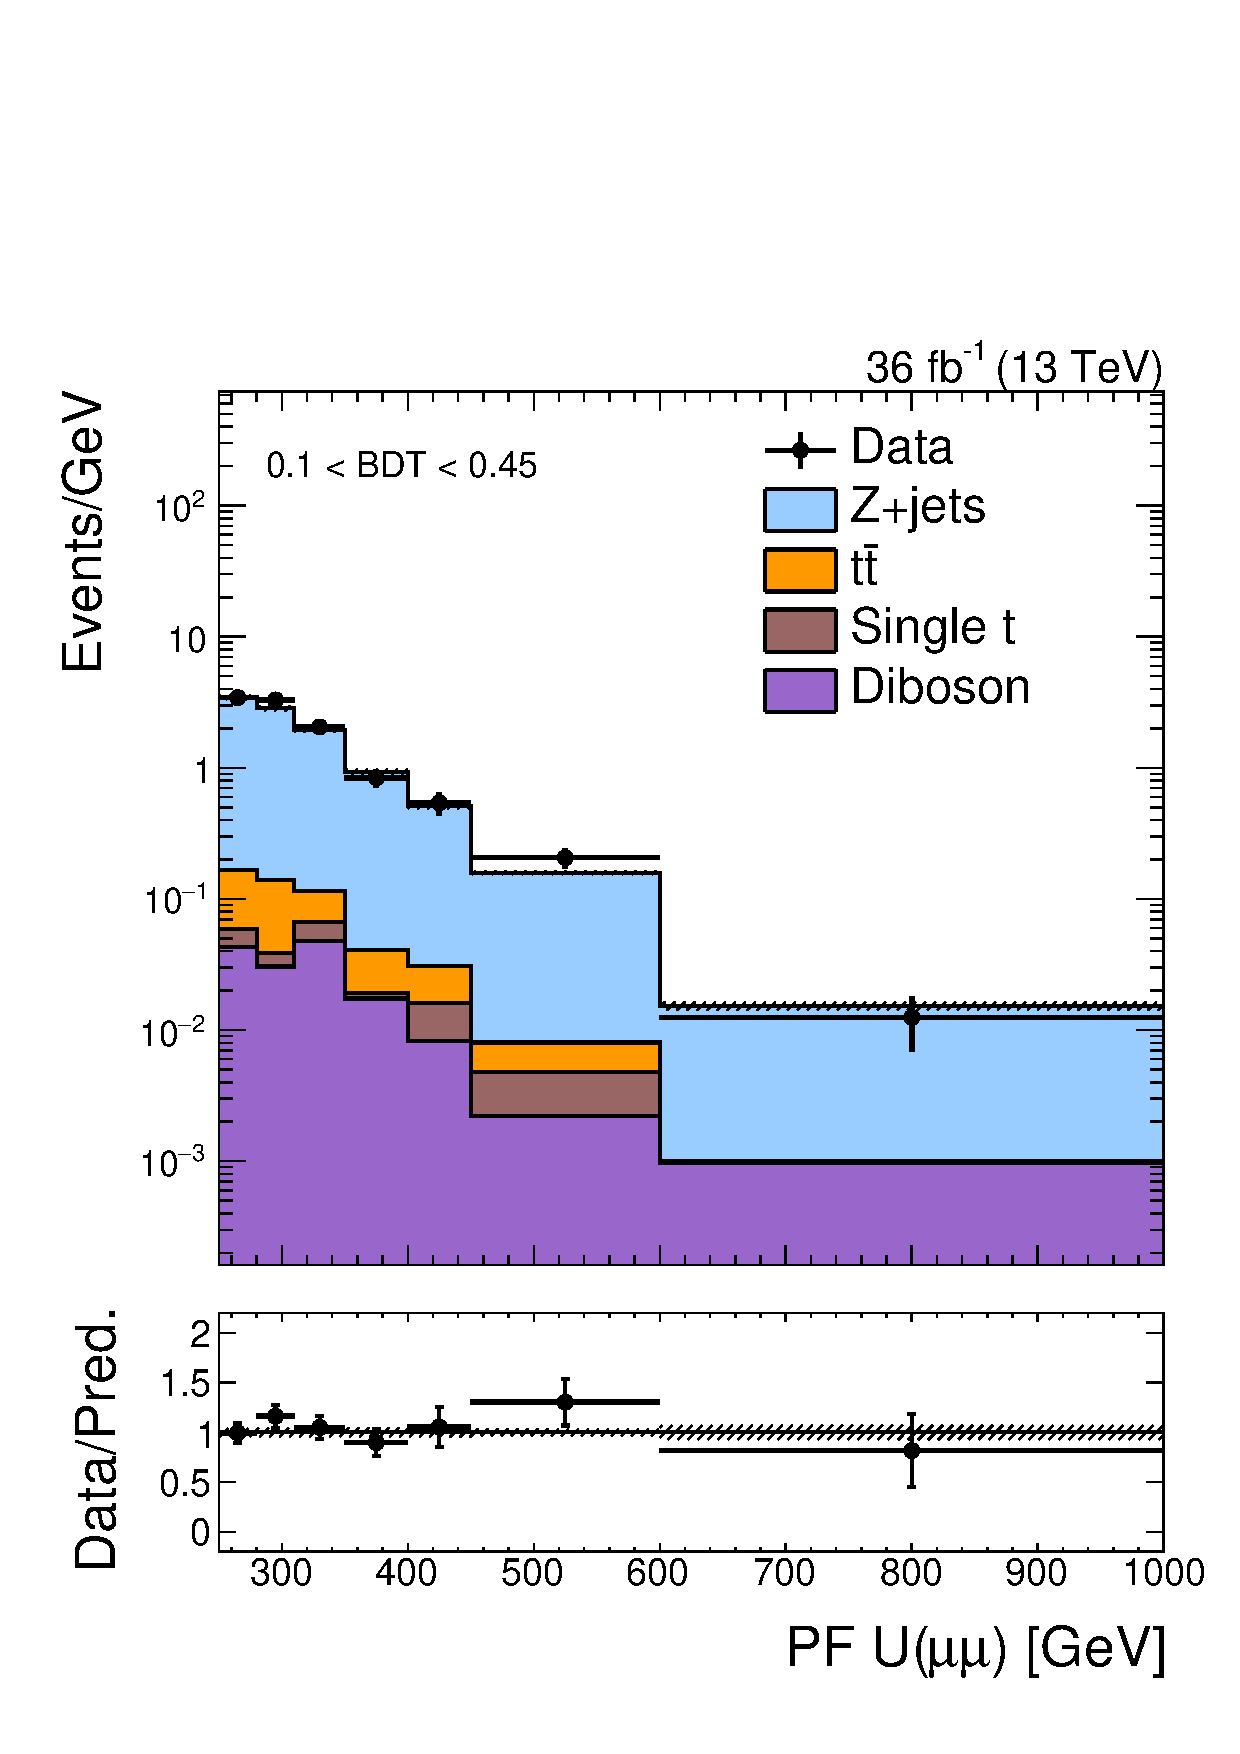
\includegraphics[width=\textwidth]{figures/monotop/prefit/dimuon_loose_pfUZmag_logy.pdf}
            \caption{Loose SR}
        \end{subfigure}
        \begin{subfigure}[t]{0.49\textwidth}
            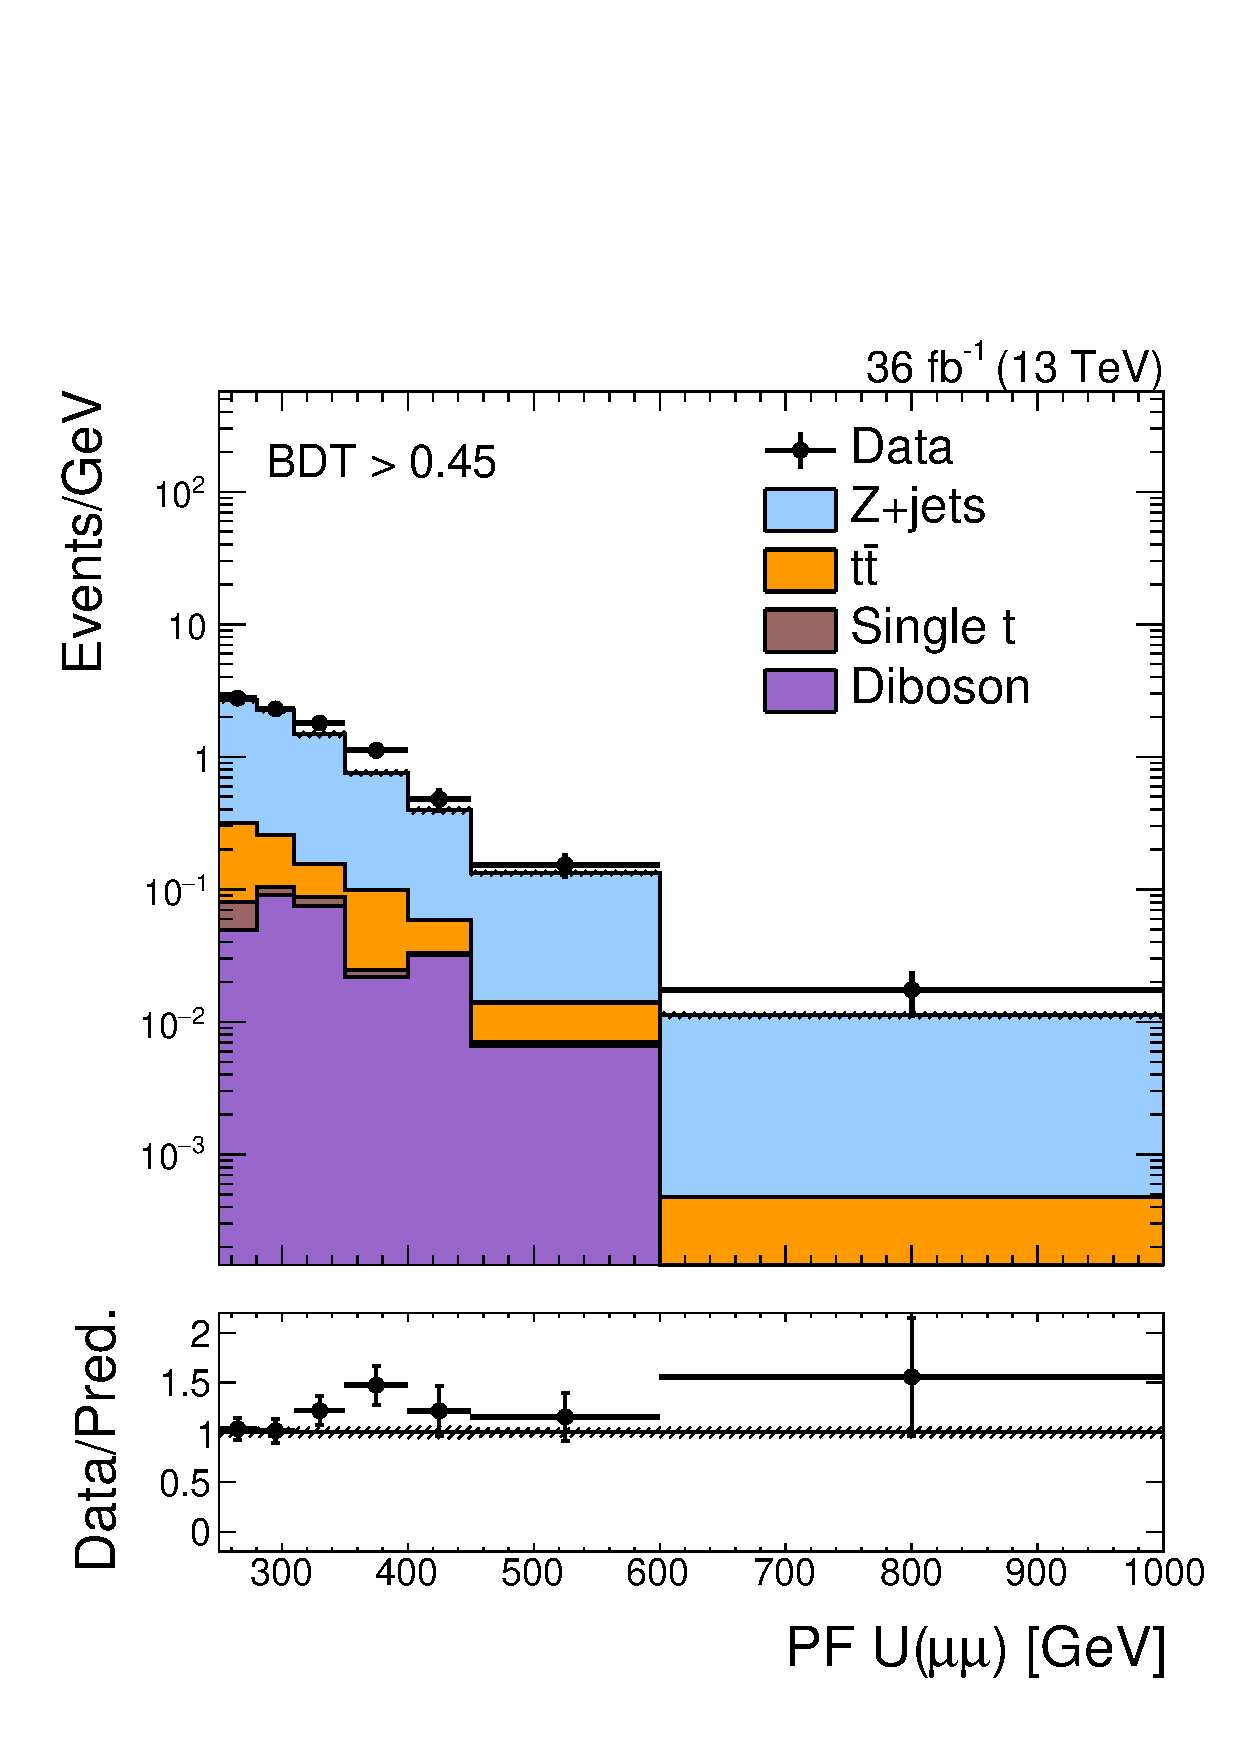
\includegraphics[width=\textwidth]{figures/monotop/prefit/dimuon_tight_pfUZmag_logy.pdf}
            \caption{Tight SR}
        \end{subfigure}
        \caption{$\ptmiss$ distributions in the two mono-top $\mu\mu$ CRs.
                 The bottom section of each figure shows the ratio of the data and the prediction.
                 The only uncertainties plotted in these figures are those arising from Poisson fluctuations in data (black bars) and MC (grey band).}
        \label{fig:mt:prefit_dimuons}
    \end{center}
\end{figure}

The control data is used to constrain the SR prediction by means of ``transfer factors'' $T^X_i$, where $X$ refers to a particular CR (e.g. $\mu\mu$) and $i$ refers to a particular bin in the CR (e.g. $200<U<250$ GeV in the tight category).
Formally:
\begin{equation}
    T^{\mu\mu}_i = \frac{N^{\mu\mu}_i(Z\rightarrow\mu\mu)}{N^\mathrm{SR}_i(Z\rightarrow\nu\nu)}
\end{equation}
The transfer factors are estimated using MC simulation.
To encode the effects of various uncertainties, we introduce nuisance parameters $\bm{\theta}$.
That is:
\begin{gather}
    T^X_i \rightarrow T^X_i(\bm\theta) \equiv T^X_i \times \prod_{j=0}^{n_\theta} (1+\theta_j) \\ 
    \theta_j \sim p(\theta_j) 
\end{gather}
where $n_\theta$ is the number of nuisance parameters and $p(\theta_j)$ is some prior distribution for each nuisance (see below for how the priors are used).
The priors are typically chosen to have a central value (e.g. mean, median) at $0$, with a finite variance that encodes the uncertainty.
In this chapter, we assume $p$ is either a normal distribution centered at 0 or a log-normal distribution (in cases where negative values are undesirable). 

Let $\pois(d|\lambda)$ refer to the Poisson probability of observing $d$ with an expected mean of $\lambda$. 
In terms of these transfer factors, the likelihood for the data observed in the signal and control regions is:
\begin{align}
    \mathcal{L}(\bm{d} | \mu, \bm{\mu}^{Z\rightarrow\nu\nu}_\mathrm{SR},  \bm{\theta}) = & \prod_{i\in\mathrm{bins}} \Big[ 
         \pois\left(d_{\mathrm{SR},i} ~|~ \mu S_{\mathrm{SR},i}(\bm\theta)  + \mu_{\mathrm{SR},i}^{Z\rightarrow\nu\nu} + B_{\mathrm{SR},i}(\bm\theta)\right) \nonumber \\
         & \phantom{\prod_{i\in\mathrm{bins}}\Big[} \times \pois\left(d_{\mu\mu,i}~|~ \mu_{\mathrm{SR},i}^{Z\rightarrow\nu\nu} \cdot T_i^{\mu\mu}(\bm\theta) + B_{\mu\mu,i}(\bm\theta) \right)\Big]  \times  \prod_{j=0}^{n_\theta} p(\theta_j)
\end{align}
where the following notation is used:
\begin{itemize}
    \item[$d_{X,i}$]: The data observed in bin $i$ of region $X$. For now, $X=\mathrm{SR},\mu\mu$. 
    \item[$S_{\mathrm{SR},i}$]: The predicted number of signal events in bin $i$ of the SR, under some fixed signal hypothesis. 
    \item[$\mu$]: The ``signal strength''. Essentially an unconstrained nuisance parameter that scales up or down the total signal yield. 
    \item[$\mu_{\mathrm{SR},i}^P$]: The expected number of events from process $P$ in bin $i$ of the SR. This is also an unconstrained nuisance parameter. 
    \item[$B_{X,i}$]: The predicted number of ``minor'' background events in bin $i$ of region $X$. Here, ``minor'' refers to all SM processes that are not the signal and are not estimated using a data-driven method. 
\end{itemize}
The signal and background yields $\bm{S}$ and $\bm{B}$ are estimated using MC.
Note that the inclusion of the priors in the likelihood constrains the nuisance parameters to be close to their ``nominal'' values; moving a $\theta_j$ to fit the data incurs a large cost from the prior.

If we set $B_i = \mu = 0$ (the null hypothesis, ignoring small minor backgrounds), then there is a simple picture of how the likelihood is maximized.
The parameters $\muz$ are float freely to satisfy $d_\mathrm{SR,i} \sim \muzi$ and $d_\mathrm{\mu\mu,i}\sim \muzi \cdot T_i^\mu\mu(\bm\theta)$. 
If both constraints cannot be satisfied simultaneously by scaling $\muz$, the (constrained) nuisance parameters $\bm\theta$ modify the transfer factor $T_i^{\mu\mu}$. 
Table~\ref{tab:mt:zmm_uncs} shows the relevant uncertainties for $T_i^{\mu\mu}$, and Fig~\ref{fig:mt:zmm_uncs} shows the shape of uncertainties that evolve as a function of $U$.

\begin{table}[!ht]
    \begin{center}
    \caption{Uncertainties affecting the $\mu\mu$ $\leftrightarrow$ $\nu\nu$ extrapolation. ``Shape'' uncertainties have different priors for each bin, but are assumed to be correlated across bins. ``Shape, uncorrelated'' uncertainties have different priors and are assumed to be uncorrelated.}
    \label{tab:mt:zmm_uncs}
    \begin{tabular}{lcl}
        Uncertainty & 1 s.d. & Notes \\ 
        \hline \hline 
        $\mu$ ID  & 2\% & \\ 
        $\mu$ track  & 1\% & \\ 
        $\tau_\mathrm{h}$ veto  & 3\% & \\ 
        $Z$+heavy flavor & 3\% & \\ 
        Trigger & 0-2\% & Shape \\ 
        $b$-tag & $\sim0.5\%$ & Shape \\ 
        $udcsg$-mistag & 3-4\% & Shape \\ 
    \end{tabular}
\end{center}
\end{table}


\begin{figure}[!ht]
    \begin{center}
        \begin{subfigure}[t]{0.49\textwidth}
            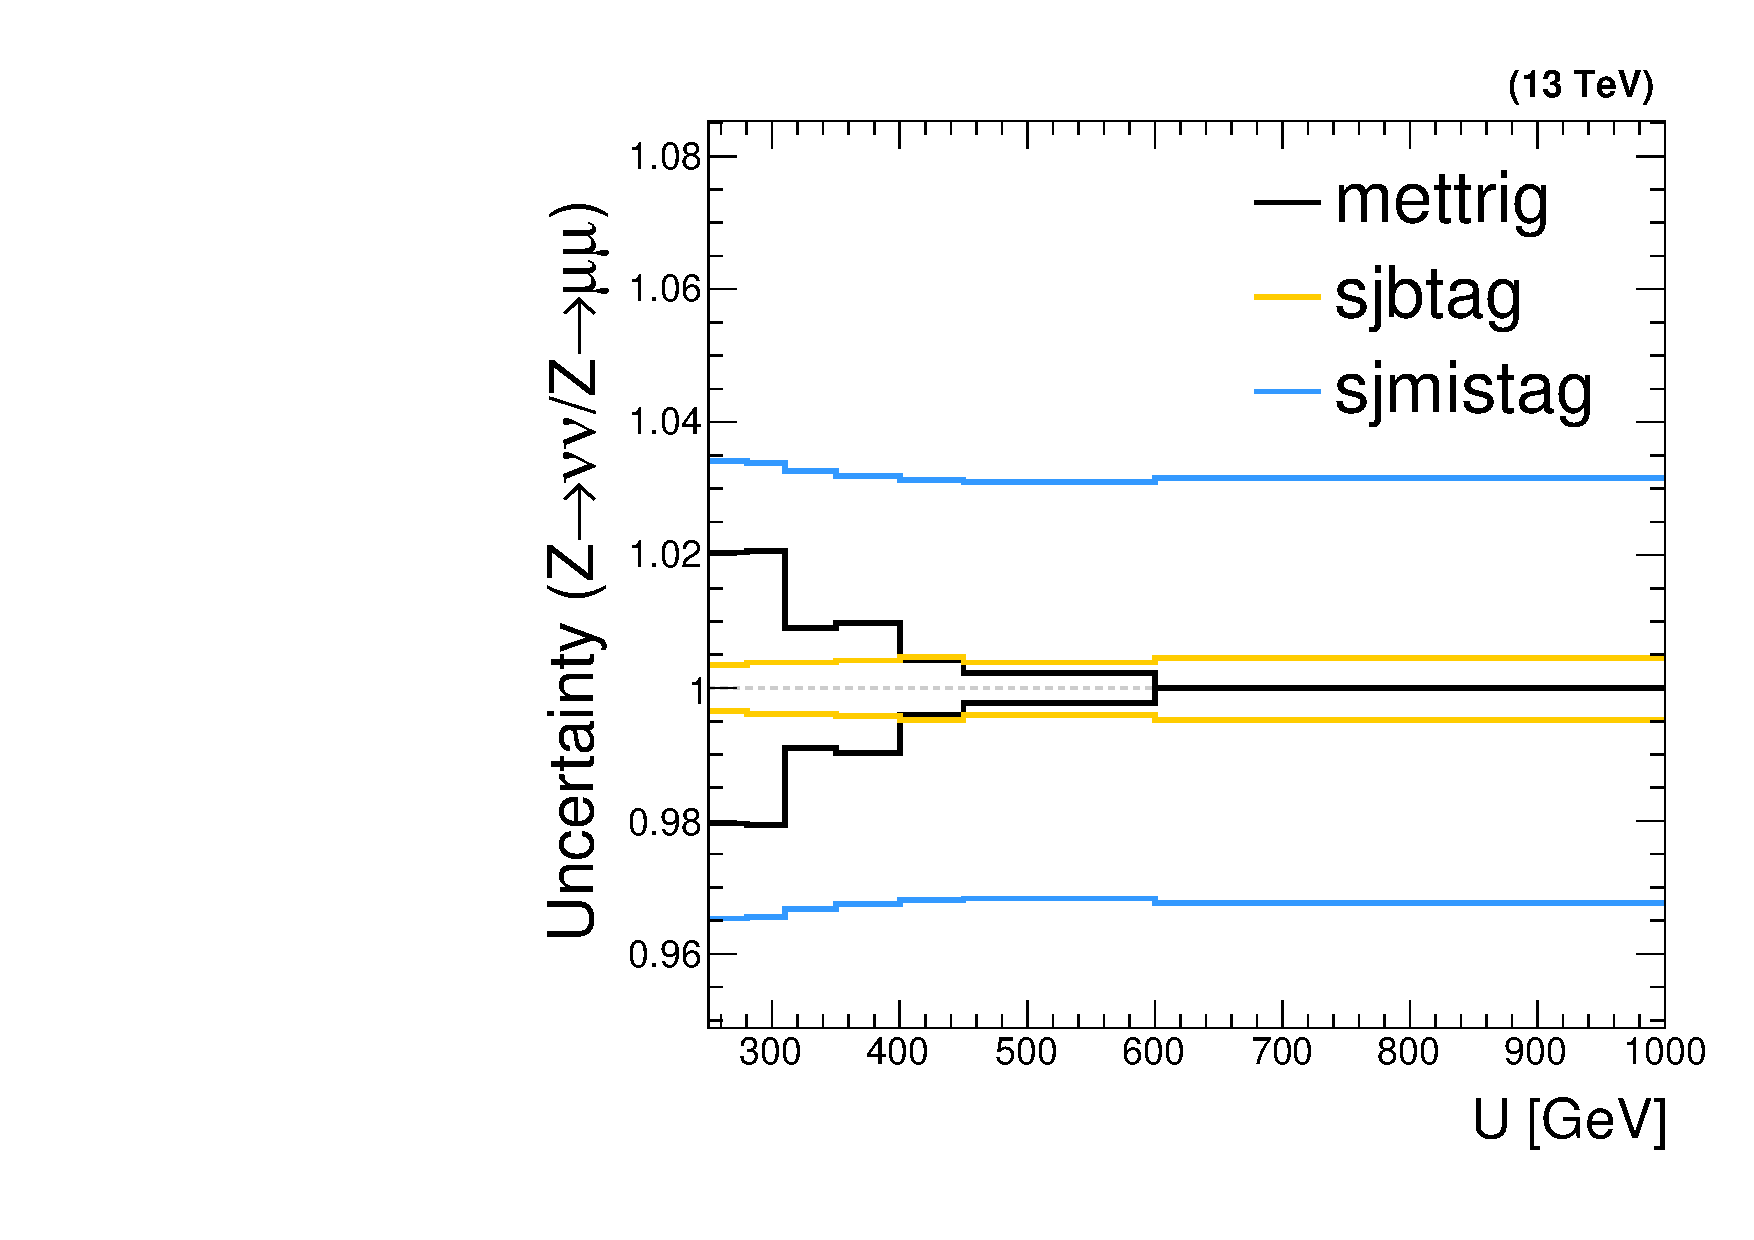
\includegraphics[width=\textwidth]{figures/monotop/uncertainties/variations_dimuon_loose.pdf}
            \caption{Loose}
        \end{subfigure}
        \begin{subfigure}[t]{0.49\textwidth}
            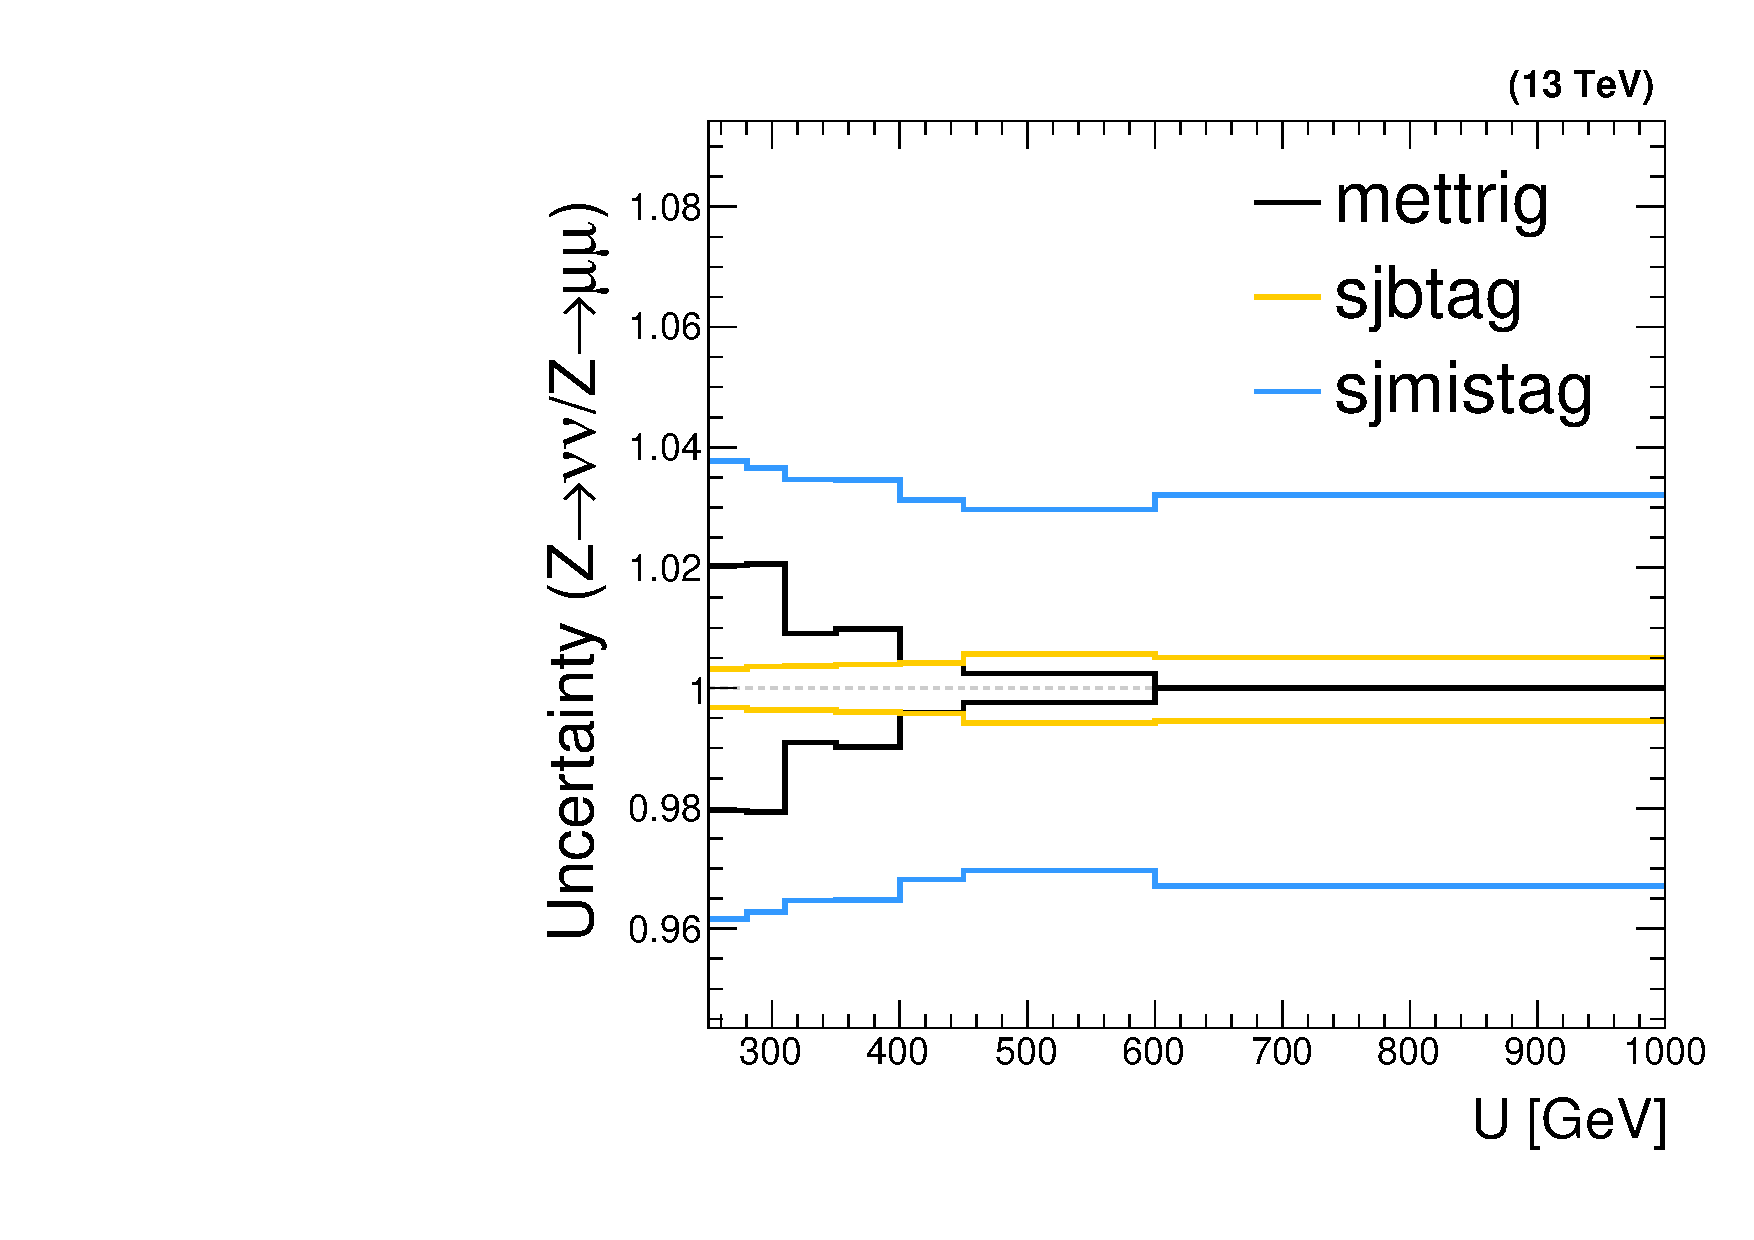
\includegraphics[width=\textwidth]{figures/monotop/uncertainties/variations_dimuon.pdf}
            \caption{Tight}
        \end{subfigure}
        \caption{Shape uncertainties affecting $T_i^{\mu\mu}$ in both categories, as a function of $U$.}
        \label{fig:mt:zmm_uncs}
    \end{center}
\end{figure}



\subsection{Theoretically-limited extrapolations}

\section{Results}

\subsection{Constraints on spin-1 FCNCs}

\subsection{Constraints on scalar resonances}

\subsection{Extending to new BSM models}
